\documentclass{beamer}

\usefonttheme{professionalfonts} % using non standard fonts for beamer
\usefonttheme{serif} % default family is serif

\usepackage{hyperref}
%\usepackage{minted}
\usepackage{animate}
\usepackage{graphicx}
\def\Put(#1,#2)#3{\leavevmode\makebox(0,0){\put(#1,#2){#3}}}
\usepackage{colortbl}
\usepackage{tikz}
\usepackage{amssymb}
\usepackage{enumerate}
\usepackage{arydshln}
\usepackage{algorithm}
\usepackage{algpseudocode}

\colorlet{lightred}{red!25}
\colorlet{lightgreen}{green!25}


\newcommand\blfootnote[1]{%

  \begingroup

  \renewcommand\thefootnote{}\footnote{#1}%

  \addtocounter{footnote}{-1}%

  \endgroup

}

\makeatletter

%%%%%%%%%%%%%%%%%%%%%%%%%%%%%% Textclass specific LaTeX commands.

 % this default might be overridden by plain title style

 \newcommand\makebeamertitle{\frame{\maketitle}}%

 % (ERT) argument for the TOC

 \AtBeginDocument{%

   \let\origtableofcontents=\tableofcontents

   \def\tableofcontents{\@ifnextchar[{\origtableofcontents}{\gobbletableofcontents}}

   \def\gobbletableofcontents#1{\origtableofcontents}

 }

%%%%%%%%%%%%%%%%%%%%%%%%%%%%%% User specified LaTeX commands.

\usetheme{Malmoe}

% or ...

\useoutertheme{infolines}

\addtobeamertemplate{headline}{}{\vskip2pt}

\setbeamercovered{transparent}

% or whatever (possibly just delete it)

\makeatother

\begin{document}
\title[PFLOCK report]{PFLOCK Report}
\author[AC]{Andres Calderon}
\institute[Winter'20]{University of California, Riverside}
\makebeamertitle
\newif\iflattersubsect

\AtBeginSection[] {
    \begin{frame}<beamer>
    \frametitle{Outline} 
    \tableofcontents[currentsection]  
    \end{frame}
    \lattersubsectfalse
}

\AtBeginSubsection[] {
    \begin{frame}<beamer>
    \frametitle{Outline} 
    \tableofcontents[currentsubsection]  
    \end{frame}
}

\begin{frame}{Finding optimal values...}
    \begin{itemize}
        \item For flock finding (Time-by-time alternative) run experiments for:
        \begin{itemize}
            \item LA\_25K dataset, $\epsilon=20$, $\mu=3$ and $\delta=3$.
            \item Evaluating first 30 time instants.
            \item Using the full cluster (12 executor, 12 cores).
        \end{itemize}
        \item Coarse grid number of partitions varying from 100 to 180...
        \item Finer grid number of partitions varying from 800 to 1200...
    \end{itemize}
\end{frame}

\begin{frame}{Finding optimal values...}
    \begin{figure}
        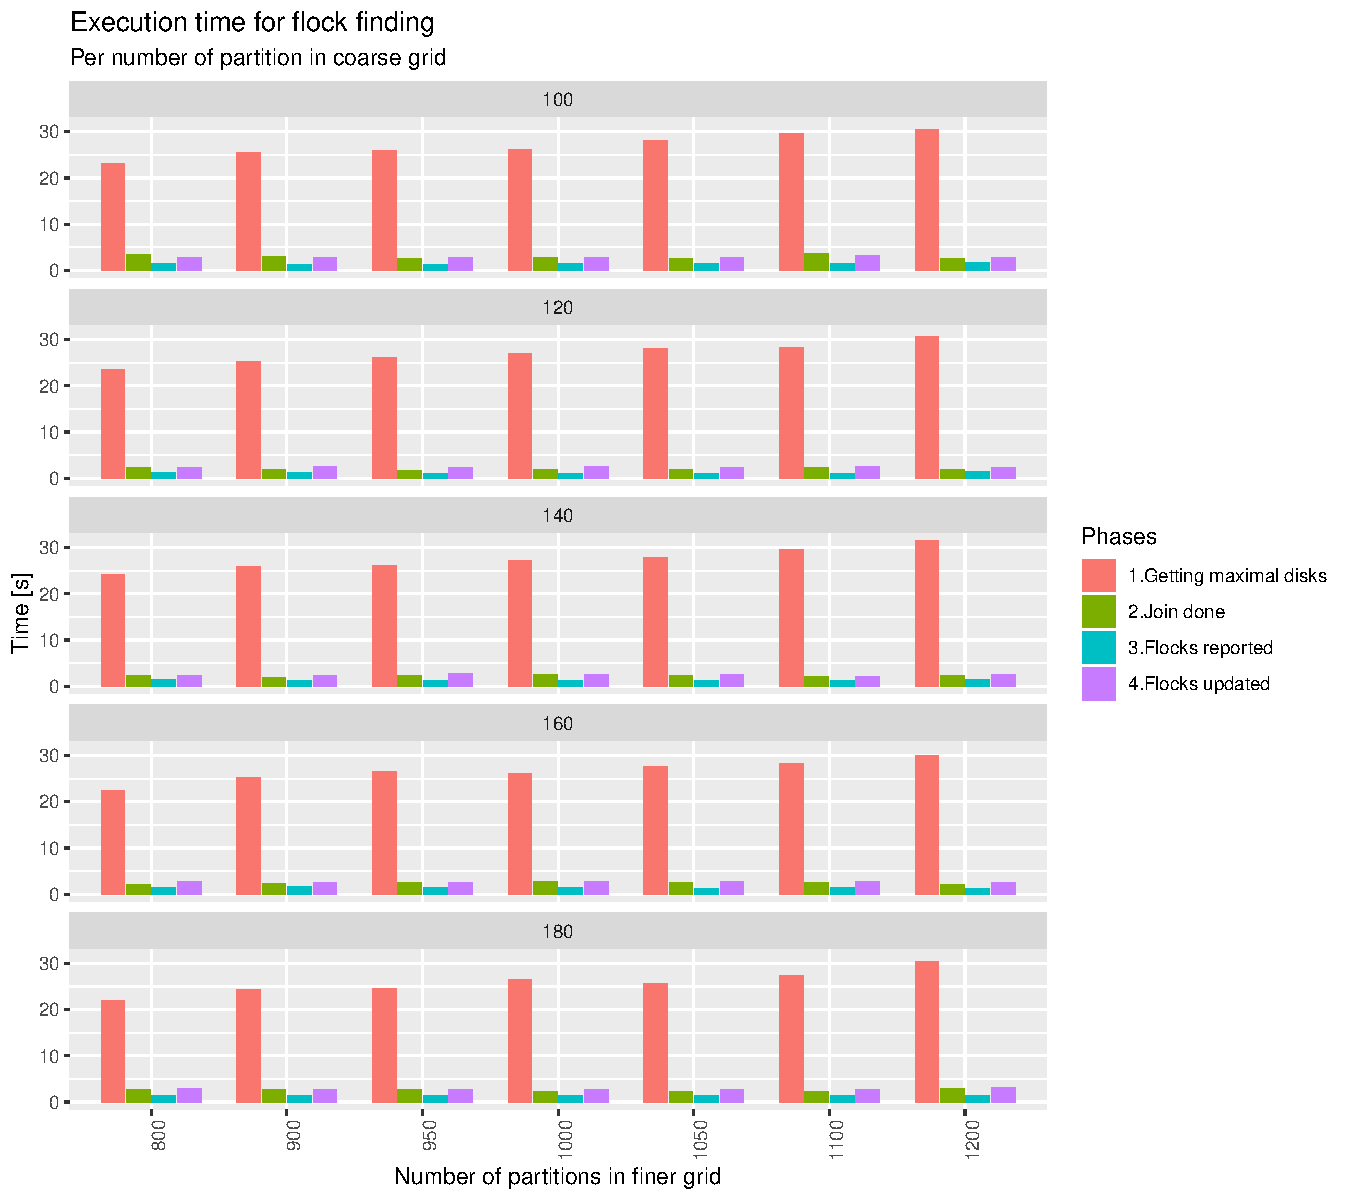
\includegraphics[width=0.7\textwidth]{FF-data}
    \end{figure}
\end{frame}

\begin{frame}{Finding optimal values...}
    \begin{itemize}
        \item Focus on maximal disk finding run experiments for:
        \begin{itemize}
            \item LA\_25K dataset. time instant 19, 3 runs...
            \item $\epsilon=20$ and $\mu=3$ 
            \item Using the full cluster (12 executor, 12 cores).
        \end{itemize}
        \item Coarse grid number of partitions varying from 144 to 720 (up to 5 times the number of available cores)...
        \item Finer grid number of partitions varying from 1000 to 4000 (up to half the size of the number of disk in the time instant)...
    \end{itemize}
\end{frame}

\begin{frame}{Finding optimal values...}
    \begin{figure}
        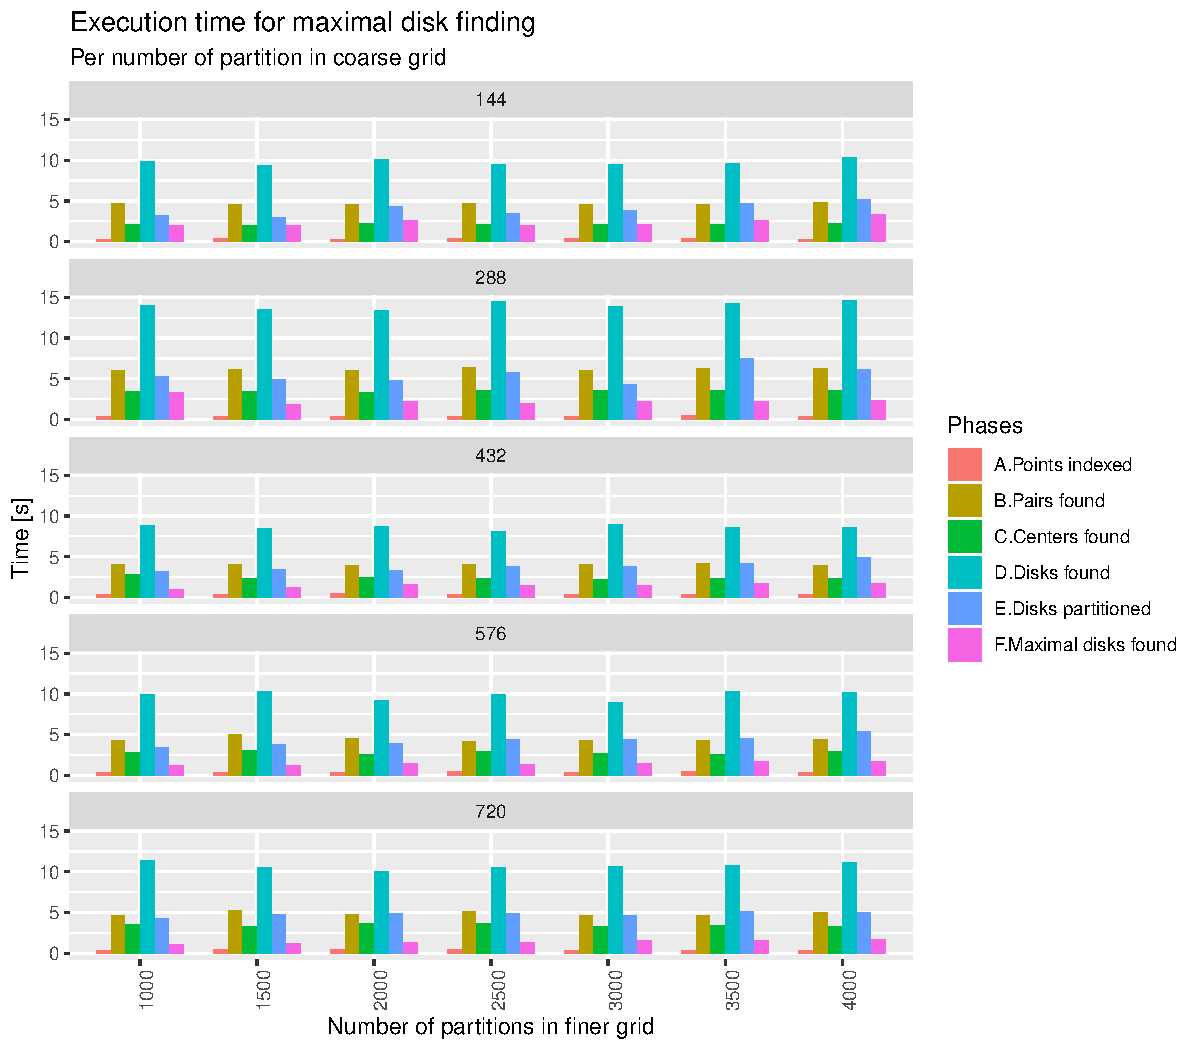
\includegraphics[width=0.7\textwidth]{MF-data}
    \end{figure}
\end{frame}

\end{document}
